\documentclass[11pt]{tex/lawoutline}
\usepackage{amssymb}
\usepackage{enumitem}

\course{Property}
\student{Prof: M. Brady}
\semester{Fall 2026}

\begin{document}

\maketitle
\tableofcontents

\chapter{Private Property and Acquisition}

\section{Acquisition Through Possession}

\definition{Acquisition Through Possession}
{
Acquisition through possession occurs when a person obtains property rights by exercising sufficient control over previously unowned property and demonstrating an intent to possess it.
}

\doctrine{First Possession}{
\begin{itemize}
    \item Mere pursuit of unowned property usually is not enough to establish possession.
    \item Possession generally requires:
    \begin{itemize}
        \item Sufficient physical control over the property; and
        \item An intent to possess or appropriate it.
    \end{itemize}
    \item The required level of control depends on the type of property and the relevant custom.
\end{itemize}
}

\subsection{Values in Declaring Possession}

\casebox
{\textit{Pierson v. Post} (1805)}
{}
{
\textbf{Facts}
\begin{itemize}
    \item Post pursued a fox during a hunt.
    \item Pierson killed and captured the fox.
\end{itemize}

\textbf{Question}
\begin{itemize}
    \item Did pursuit alone give Post a property right in the fox?
\end{itemize}

\textbf{Holding}
\begin{itemize}
    \item No. Mere pursuit was insufficient to establish possession.
    \item Possession required capture, mortal wounding, or another act that deprived the animal of its natural liberty.
\end{itemize}

\textbf{Discussion}
\begin{itemize}
    \item The majority preferred a clear and administrable rule because pursuit is difficult to define.
    \item A rule protecting mere pursuit could generate extensive litigation over how close a pursuer was to capture.
    \item The dissent favored protecting the labor and investment involved in pursuing the fox.
    \item The case illustrates the relationship between property rules and:
    \begin{itemize}
        \item Labor;
        \item Fairness;
        \item Administrability; and
        \item Institutional capacity.
    \end{itemize}
\end{itemize}
}

\note{Levels of Analysis in \textit{Pierson}}{
\begin{enumerate}
    \item \textbf{Rule:} What conduct establishes possession?
    \item \textbf{Institutional concern:} Which rule is sufficiently clear for courts to administer?
    \item \textbf{Underlying values:} Should the law reward labor, encourage hunting, prevent litigation, or produce a fair result?
\end{enumerate}
}


\subsection{Cultural Norms of Possession}

\casebox
{\textit{Ghen v. Rich} (1881)}
{}
{
\textbf{Facts}
\begin{itemize}
    \item Ghen killed a whale using a distinctive bomb lance.
    \item The whale later washed ashore, where Ellis found and sold it to Rich.
    \item A local custom provided that the person who killed the whale retained ownership even if someone else later found it.
\end{itemize}

\textbf{Question}
\begin{itemize}
    \item Should the court apply the local custom rather than the ordinary rule that possession belongs to the finder?
\end{itemize}

\textbf{Holding}
\begin{itemize}
    \item Yes. The court recognized Ghen's ownership under the established custom of the whaling industry.
\end{itemize}

\textbf{Discussion}
\begin{itemize}
    \item Courts may defer to a custom when:
    \begin{enumerate}
        \item The custom is generally followed by members of the relevant industry;
        \item It has existed for a substantial period of time;
        \item It promotes desirable economic or social outcomes; and
        \item It is limited to a defined group or activity.
    \end{enumerate}
    \item Applying the custom protected the whaling industry and encouraged people to undertake the costly labor of hunting whales.
    \item The case illustrates that possession rules may be shaped by industry-specific practices rather than a universal physical-capture rule.
\end{itemize}
}

\subsection{Noncompetitive Possession}

\casebox
{\textit{Keeble v. Hickeringill} (1707)}
{}
{
\textbf{Facts}
\begin{itemize}
    \item Keeble operated a decoy pond to attract and capture wild ducks.
    \item Hickeringill intentionally fired guns to scare the ducks away.
    \item Hickeringill did not seek to capture the ducks himself.
\end{itemize}

\textbf{Holding}
\begin{itemize}
    \item Keeble could recover for the intentional interference with his lawful use of the pond.
\end{itemize}

\textbf{Discussion}
\begin{itemize}
    \item Keeble did not own the wild ducks merely because they visited his land.
    \item Nevertheless, he had a protected interest in using his land and business to pursue them.
    \item The law distinguishes between:
    \begin{itemize}
        \item Legitimate competition for a resource; and
        \item Malicious interference intended only to prevent another person from obtaining it.
    \end{itemize}
    \item The case protects productive uses of property and discourages spiteful interference.
\end{itemize}
}


\subsection{Limits of Possession}

\casebox
{\textit{Popov v. Hayashi} (2002)}
{}
{
\textbf{Facts}
\begin{itemize}
    \item Popov caught Barry Bonds's record-setting baseball, but a crowd caused him to lose control before he fully secured it.
    \item Hayashi recovered the ball after it left Popov's possession.
\end{itemize}

\textbf{Question}
\begin{itemize}
    \item Did either Popov or Hayashi have a superior possessory claim to the ball?
\end{itemize}

\textbf{Holding}
\begin{itemize}
    \item Popov had a legally cognizable pre-possessory interest because he had taken significant steps toward possession and lost control because of the unlawful acts of others.
    \item Hayashi also acquired a possessory interest by obtaining physical control of the ball.
    \item The court divided the proceeds equally.
\end{itemize}

\textbf{Discussion}
\begin{itemize}
    \item The case recognizes an interest that exists between mere pursuit and complete possession.
    \item The remedy reflected fairness and equal distribution rather than a simple winner-take-all rule.
    \item Hayashi did not cause Popov to lose control of the ball, which supported treating both parties as having legitimate interests.
\end{itemize}
}

\definition{Trespass to Chattels}
{
An intentional interference with another person's possession of personal property that causes dispossession, impairment, or deprivation of use.
}

\definition{Chattel}{Any item of movable personal property that is distinct from real estate or land.}

\definition{Conversion}
{
An intentional exercise of control over another person's property that is sufficiently serious to justify requiring the defendant to pay the property's full value.
}

\subsection{Takeaways}{
\begin{enumerate}
    \item Possession rules are often designed to be administrable rather than perfectly precise.
    \item Courts may recognize custom when ordinary possession rules would undermine a particular industry.
    \item Property law protects productive use even when the claimant does not own the resource itself.
    \item Courts may use equitable remedies when rigid possession rules would produce an unfair result.
\end{enumerate}
}


\section{Acquisition Through Discovery}

\definition{Acquisition Through Discovery}
{
Discovery is a method of acquiring title in which a sovereign claims ownership or superior title over land based on being the first European power to discover or conquer the territory.
}

\doctrine{Discovery Doctrine}{
\begin{itemize}
    \item Under the discovery doctrine, European sovereigns acquired superior title to lands they ``discovered.''
    \item Indigenous peoples retained a right of occupancy, but that right could be extinguished by:
    \begin{itemize}
        \item Treaty;
        \item Conquest; or
        \item The discovering sovereign's decision to transfer the land.
    \end{itemize}
    \item The doctrine illustrates how property law can reflect and enforce political power.
\end{itemize}
}

\definition{\textit{Nemo Dat}}
{
No person can transfer better title than that person possesses. In the context of Native American land, however, the discovery doctrine treated the United States as holding superior title even when Indigenous groups retained occupancy rights.
}

\subsection{Native American Property}

\casebox
{\textit{Johnson v. M'Intosh} (1823)}
{}
{
\textbf{Facts}
\begin{itemize}
    \item Johnson claimed title based on land purchases from Native American tribes.
    \item M'Intosh claimed title based on a later grant from the United States government.
\end{itemize}

\textbf{Question}
\begin{itemize}
    \item Did the tribal conveyances give Johnson a title enforceable in United States courts?
\end{itemize}

\textbf{Holding}
\begin{itemize}
    \item No. The Court held that the United States held superior title under the discovery doctrine.
    \item The tribes retained a right of occupancy but could not transfer ultimate title to private individuals.
\end{itemize}

\textbf{Discussion}
\begin{itemize}
    \item The decision shows how property law can be used instrumentally to facilitate territorial acquisition and dispossession.
    \item The Court emphasized administrability and the need for a single recognized sovereign title.
    \item The case raises questions about whether property law reflects neutral principles or the interests of the politically dominant group.
\end{itemize}
}

\note{Harvard's Acquisition of Land}{
\begin{itemize}
    \item The history of property acquisition raises questions about how universities and other institutions acquired land.
    \item These questions connect property doctrine to:
    \begin{itemize}
        \item Historical injustice;
        \item Political power;
        \item Institutional responsibility; and
        \item Possible remedies.
    \end{itemize}
\end{itemize}
}

\subsection{Cultural Patrimony and Human Remains}

\rulebox{NAGPRA and Cultural Patrimony}{
Under NAGPRA, an object may qualify as protected cultural patrimony when:
\begin{enumerate}
    \item It is not owned by an individual tribal member;
    \item It is considered inalienable; and
    \item It has an ongoing historical, traditional, or cultural importance central to the Native American group.
\end{enumerate}
}

\casebox
{\textit{United States v. Corrow}}
{}
{
\textbf{Facts}
\begin{itemize}
    \item Corrow purchased Navajo ceremonial masks and attempted to resell them for profit.
    \item The government prosecuted him under NAGPRA.
\end{itemize}

\textbf{Holding}
\begin{itemize}
    \item The masks were cultural patrimony because they were centrally important to the Navajo community and could not be privately alienated by an individual member.
\end{itemize}

\textbf{Discussion}
\begin{itemize}
    \item Property may be communal rather than individually owned.
    \item Tribal custom may determine whether an object is alienable.
    \item NAGPRA limits ordinary market-based assumptions about ownership and transfer.
\end{itemize}
}

\subsection{Custom and Tribal Law}

\casebox
{\textit{Smith v. James}}
{}
{
\textbf{Facts}
\begin{itemize}
    \item The dispute concerned Hopi rules governing the transfer of land within the community.
    \item The relevant customs involved questions of family status, residence, and the role of community members.
\end{itemize}

\textbf{Holding}
\begin{itemize}
    \item The court ordered a hearing involving village members and witnesses familiar with Hopi custom before determining the governing legal rule.
\end{itemize}

\textbf{Discussion}
\begin{itemize}
    \item Courts may not be the best institution to determine the content of Indigenous legal customs without consulting the relevant community.
    \item The case illustrates the interaction between Western courts and Indigenous legal systems.
    \item Custom may be identified through community-based testimony rather than solely through written legal sources.
\end{itemize}
}

\subsection{Takeaways}{
\begin{enumerate}
    \item Discovery and conquest demonstrate the relationship between property and political power.
    \item Property law can be used to recognize, deny, or restructure Indigenous possessory rights.
    \item NAGPRA protects certain forms of communal and inalienable property.
    \item Custom may be an important source of property law, but courts must consider who has the authority to define the custom.
\end{enumerate}
}


\section{Acquisition Through Creation}

\note{Creation and Property Rights}{
\begin{itemize}
    \item Property rights in creations may be justified by:
    \begin{itemize}
        \item Labor and desert;
        \item Incentives to create and innovate;
        \item Fairness to the creator;
        \item Economic efficiency; and
        \item The need to encourage socially valuable production.
    \end{itemize}
    \item Creation-based property rights are limited when exclusive rights would:
    \begin{itemize}
        \item Restrict public access;
        \item Suppress speech or competition;
        \item Create excessive monopoly power;
        \item Protect facts or ideas rather than expression; or
        \item Exceed the institutional capacity of courts.
    \end{itemize}
\end{itemize}
}

\subsection{Right to Publicity}

\definition{Right of Publicity}
{
The right to control the commercial use of one's name, image, likeness, voice, or other identifying characteristics.
}

\doctrine{Right of Publicity}{
\begin{itemize}
    \item The right of publicity varies by state.
    \item It generally protects against unauthorized commercial appropriation of a person's identity.
    \item The claim is strongest when:
    \begin{itemize}
        \item The defendant uses an identity-related characteristic;
        \item The use is intended to evoke the particular person; and
        \item The use is connected to commercial advertising or profit.
    \end{itemize}
    \item The right does not necessarily apply to informative, cultural, or expressive uses.
\end{itemize}
}

\casebox
{\textit{Midler v. Ford Motor Co.} (1988)}
{}
{
\textbf{Facts}
\begin{itemize}
    \item Ford used a singer who imitated Bette Midler's distinctive voice in a commercial.
    \item Midler had not authorized the use.
\end{itemize}

\textbf{Holding}
\begin{itemize}
    \item The use of a distinctive voice to imitate Midler for commercial purposes could constitute an unlawful appropriation of her identity.
\end{itemize}

\textbf{Discussion}
\begin{itemize}
    \item The defendant did not use Midler's name or literal image, but intentionally copied a distinctive identity-related characteristic.
    \item The case treats the voice as a property-like interest connected to Midler's labor and public identity.
    \item It raises questions about whether creators should control uses that imitate their work or persona, including through AI.
\end{itemize}
}

\casebox
{\textit{White v. Samsung Electronics America, Inc.} (1992)}
{}
{
\textbf{Facts}
\begin{itemize}
    \item Samsung used an advertisement featuring a robot dressed and posed in a way that evoked Vanna White.
    \item The advertisement did not use White's literal name or photograph.
\end{itemize}

\textbf{Holding}
\begin{itemize}
    \item White could pursue a right-of-publicity claim because the advertisement appropriated her identity even without using her exact likeness.
\end{itemize}

\textbf{Discussion}
\begin{itemize}
    \item Context matters when determining whether an image evokes a particular person.
    \item The dissent warned that an expansive right of publicity could restrict parody, creativity, and public discourse.
    \item The case illustrates the tension between protecting identity and allowing others to build on existing cultural images.
\end{itemize}
}

\casebox
{\textit{Lanier v. President and Fellows of Harvard College}}
{}
{
\textbf{Facts}
\begin{itemize}
    \item The case involved photographs of enslaved people taken roughly a century earlier and later held by Harvard.
    \item A descendant sought to assert an interest based on the photographed person's identity.
\end{itemize}

\textbf{Holding}
\begin{itemize}
    \item The court did not recognize a right-of-publicity claim belonging to the descendant based on the historical photographs.
\end{itemize}

\textbf{Discussion}
\begin{itemize}
    \item The case illustrates the limits of extending modern property rights backward in time.
    \item The court emphasized institutional capacity and declined to create a new cause of action through judicial decision.
    \item The dispute raises questions about whether moral wrongs should be addressed through property law, legislation, restitution, or another remedy.
\end{itemize}
}

\subsection{Copyright}

\definition{Copyright}
{
Copyright protects original works of authorship that are fixed in a tangible medium of expression.
}

\commonlaw{Copyright Requirements}{
\begin{itemize}
    \item The work must be:
    \begin{enumerate}
        \item An original work of authorship;
        \item Fixed in a tangible medium; and
        \item Sufficiently creative.
    \end{enumerate}
    \item Copyright protects expression, not bare facts, ideas, or information.
    \item Copyright therefore creates a limited property right rather than complete ownership over all information associated with a work.
\end{itemize}
}

\casebox
{\textit{International News Service v. Associated Press} (1918)}
{}
{
\textbf{Facts}
\begin{itemize}
    \item International News Service copied news gathered by the Associated Press and distributed it to competing newspapers.
\end{itemize}

\textbf{Holding}
\begin{itemize}
    \item The Court recognized a limited quasi-property interest in the news as between competing news organizations.
\end{itemize}

\textbf{Discussion}
\begin{itemize}
    \item There is no general property right in news against the public.
    \item The quasi-property right applied primarily to prevent unfair competition between the parties.
    \item The decision reflected:
    \begin{itemize}
        \item Labor-desert concerns;
        \item Fairness;
        \item Incentives to gather and publish news; and
        \item The goal of preserving public access to information.
    \end{itemize}
\end{itemize}
}

\casebox
{\textit{Feist Publications v. Rural Telephone Service Co.} (1991)}
{}
{
\textbf{Facts}
\begin{itemize}
    \item Rural Telephone published a directory containing subscriber information.
    \item Feist copied the information into a larger directory.
\end{itemize}

\textbf{Holding}
\begin{itemize}
    \item Facts are not copyrightable.
    \item A compilation may be copyrightable only when its selection, coordination, or arrangement contains sufficient originality.
    \item Rural's alphabetical directory lacked the required creativity.
\end{itemize}

\textbf{Discussion}
\begin{itemize}
    \item Labor alone is not enough to obtain copyright protection.
    \item Copyright rewards original expression rather than effort expended to collect facts.
    \item The case limits exclusivity in order to preserve public access to factual information.
\end{itemize}
}

\subsubsection{Fair Use}{
\begin{itemize}
    \item Fair use limits copyright exclusivity and permits certain uses of copyrighted material.
    \item Courts consider:
    \begin{enumerate}
        \item The purpose and character of the use;
        \item The nature of the copyrighted work;
        \item The amount and substantiality of the portion used; and
        \item The effect of the use on the potential market for the copyrighted work.
    \end{enumerate}
    \item Fair use reflects the need to balance creator rights against speech, education, competition, and future creativity.
\end{itemize}
}

\subsection{Patents}

\definition{Patent}
{
A patent grants an inventor an exclusive right in a new and useful invention for a limited period of time.
}

\textbf{When should property rights arise, and in whom?}
{
\begin{itemize}
    \item Copyright generally arises in original human expression fixed in a tangible medium.
    \item Patent rights arise for qualifying inventions rather than for mere labor or discovery of something already existing in nature.
    \item Patent law generally requires:
    \begin{itemize}
        \item A new and useful process, machine, manufacture, or composition of matter;
        \item Human inventorship; and
        \item Compliance with statutory requirements.
    \end{itemize}
    \item The relevant rights may belong to the inventor, an employer, or another assignee depending on the circumstances.
\end{itemize}
}

\textbf{Justifications for awarding property rights}
{
\begin{itemize}
    \item \textbf{Labor-desert theory:} creators deserve control over the products of their labor.
    \item \textbf{Incentive theory:} exclusive rights encourage research, creation, and innovation.
    \item \textbf{Efficiency:} property rights may encourage investment and reduce duplication.
    \item \textbf{Fairness:} creators should not be deprived of the economic benefits of their work.
    \item \textbf{Personhood:} certain creations may be connected to the identity and autonomy of the creator.
\end{itemize}
}

\textbf{Policy goals invoked to limit property rights}
{
\begin{itemize}
    \item Encouraging future innovation by allowing others to build on existing ideas.
    \item Preserving public access to facts, ideas, and scientific discoveries.
    \item Preventing excessive monopoly power.
    \item Protecting free expression and parody.
    \item Avoiding protection for things that courts or legislatures lack the institutional capacity to define.
    \item Ensuring that property rights do not extend to naturally occurring phenomena or abstract ideas.
\end{itemize}
}

\casebox
{\textit{Diamond v. Chakrabarty} (1980)}
{}
{
\textbf{Facts}
\begin{itemize}
    \item Chakrabarty developed a genetically engineered microorganism capable of breaking down oil.
\end{itemize}

\textbf{Holding}
\begin{itemize}
    \item The microorganism was patentable as a ``manufacture'' or ``composition of matter'' under the Patent Act.
\end{itemize}

\textbf{Discussion}
\begin{itemize}
    \item Patent law is designed to encourage technological progress and research.
    \item The relevant question was whether the organism was a human-made invention rather than a naturally occurring product.
    \item The case shows that patent law is not based solely on labor-desert theory; it also promotes innovation.
\end{itemize}
}

\casebox
{\textit{Association for Molecular Pathology v. Myriad Genetics, Inc.} (2013)}
{}
{
\textbf{Facts}
\begin{itemize}
    \item Myriad identified and isolated DNA sequences associated with a disease.
    \item Myriad sought patents covering the isolated DNA.
\end{itemize}

\textbf{Holding}
\begin{itemize}
    \item Naturally occurring DNA is not patentable merely because it has been isolated.
    \item Complementary DNA, or cDNA, may be patentable because it is not naturally occurring.
\end{itemize}

\textbf{Discussion}
\begin{itemize}
    \item Extensive effort and discovery alone do not create a patentable invention.
    \item Patent law excludes products of nature, laws of nature, and abstract ideas.
    \item The case draws a boundary between human invention and discovery of something already existing in nature.
\end{itemize}
}

\casebox
{\textit{Thaler v. Vidal}}
{}
{
\textbf{Facts}
\begin{itemize}
    \item Thaler attempted to list an artificial-intelligence system as the inventor of an invention.
\end{itemize}

\textbf{Holding}
\begin{itemize}
    \item The Patent Act requires an inventor to be a natural person.
    \item An AI system cannot be listed as the inventor.
\end{itemize}

\textbf{Discussion}
\begin{itemize}
    \item The case raises questions about whether innovation-based property rights should be awarded to machines, their owners, or human developers.
    \item The court relied on statutory language rather than creating a new category of AI inventorship.
\end{itemize}
}

\casebox
{\textit{Thaler v. Perlmutter}}
{}
{
\textbf{Facts}
\begin{itemize}
    \item Thaler sought copyright protection for an image generated entirely by an artificial-intelligence system.
\end{itemize}

\textbf{Holding}
\begin{itemize}
    \item A machine cannot be the author of a copyrighted work.
    \item Copyright requires human authorship.
\end{itemize}

\textbf{Discussion}
\begin{itemize}
    \item Copyright law rewards human creativity and authorship.
    \item The decision leaves open questions about works involving substantial human input and AI assistance.
\end{itemize}
}

\casebox
{\textit{Bartz v. Anthropic}}
{}
{
\textbf{Facts}
\begin{itemize}
    \item Authors alleged that Anthropic used books to train an AI system without authorization.
\end{itemize}

\textbf{Discussion}
\begin{itemize}
    \item The dispute illustrates how traditional fair-use factors apply to AI training.
    \item Important questions include:
    \begin{itemize}
        \item Whether the purpose of training is sufficiently transformative;
        \item Whether the works used are expressive;
        \item How much of the works were copied; and
        \item Whether AI training harms the market for the original works.
    \end{itemize}
\end{itemize}
}

\casebox
{\textit{Thomson Reuters v. Ross Intelligence}}
{}
{
\textbf{Facts}
\begin{itemize}
    \item Ross allegedly used Thomson Reuters' legal headnotes to develop an AI legal research system.
\end{itemize}

\textbf{Holding}
\begin{itemize}
    \item The headnotes were sufficiently original to receive copyright protection.
\end{itemize}

\textbf{Discussion}
\begin{itemize}
    \item The headnotes reflected creative selection, synthesis, and explanation of legal opinions.
    \item The case demonstrates that even material based on public-domain judicial opinions may be protected when the selection and expression contain sufficient originality.
\end{itemize}
}

\note{Creation-Based Property Takeaways}{
\begin{itemize}
    \item Different intellectual-property regimes reward different interests:
    \begin{itemize}
        \item Copyright rewards original expression;
        \item Patent law rewards qualifying inventions; and
        \item The right of publicity protects commercial control over identity.
    \end{itemize}
    \item Each regime also limits exclusivity to protect public access, competition, speech, and future innovation.
    \item AI exposes difficult questions about:
    \begin{itemize}
        \item Human authorship and inventorship;
        \item Training data;
        \item Style imitation;
        \item Originality; and
        \item The proper recipient of property rights.
    \end{itemize}
\end{itemize}
}


\section{Acquisition Through Adverse Possession}

\doctrine{Adverse Possession}
{
If the true owner does not timely assert ownership rights while another person openly treats the land as their own, the law may eventually recognize the possessor as the owner.
}

\subsection{Purposes of Adverse Possession}{
\begin{itemize}
    \item \textbf{Quiet title:} resolves uncertainty about ownership.
    \item \textbf{Encouraging productive use:} rewards people who use and improve neglected land.
    \item \textbf{Penalizing sleeping owners:} encourages owners to monitor and assert their rights.
    \item \textbf{Reliance and personhood:} protects possessors who develop an attachment to and invest in the property.
    \item \textbf{Administrative efficiency:} reduces the difficulty of resolving very old disputes over land boundaries and title.
    \item \textbf{Land circulation:} moves property toward people who are actively using it.
\end{itemize}
}

\subsection{Elements of Adverse Possession}

\rulebox{Requirements for Adverse Possession}{
To constitute adverse possession, possession generally must be:

\begin{enumerate}
    \item \textbf{Actual:} The possessor engages in acts that resemble the ordinary use of an owner.
    
    \item \textbf{Exclusive:} The possessor uses the land in a way that is inconsistent with possession by the true owner, the public, or other adverse possessors.
    
    \item \textbf{Continuous:} The possession continues for the statutory period. Continuity does not require constant daily use; the possessor must use the property as an ordinary owner would, given its nature.
    
    \item \textbf{Open and notorious:} The possession is sufficiently visible that a reasonable owner would have notice of it.
    
    \item \textbf{Hostile under a claim of right:}
    \begin{itemize}
        \item \textbf{Hostile:} The possession is without permission or after permission has been revoked.
        \item \textbf{Claim of right:}
        \begin{itemize}
            \item Under an objective test, the possession must appear to be a claim of ownership.
            \item Under a subjective test, the possessor must have a good-faith belief that they have a legitimate claim to the land.
        \end{itemize}
    \end{itemize}
\end{enumerate}

Some jurisdictions also require that possession be peaceable. This is not a universal element.
}

\casebox
{\textit{Scott v. Anderson-Tully Co.} (2015)}
{}
{
\textbf{Facts}
\begin{itemize}
    \item Scott claimed ownership of a disputed parcel through inheritance.
    \item Anderson-Tully marked the boundary, harvested timber, and granted hunting licenses over the land.
\end{itemize}

\textbf{Question}
\begin{itemize}
    \item Did Anderson-Tully establish adverse possession?
\end{itemize}

\textbf{Holding}
\begin{itemize}
    \item Yes. Anderson-Tully established the relevant Mississippi requirements.
\end{itemize}

\textbf{Discussion}
\begin{itemize}
    \item \textbf{Actual:} Boundary marking, timber harvesting, and other uses resembled acts of ownership.
    \item \textbf{Exclusive:} Anderson-Tully used the land as its own and sought to exclude others.
    \item \textbf{Continuous:} The boundary was maintained and the land was periodically used over the statutory period.
    \item \textbf{Open and notorious:} The painted boundary and fence were visible to the community.
    \item \textbf{Hostile under a claim of right:} Anderson-Tully used the land without Scott's permission and treated it as its own.
    \item \textbf{Peaceable:} Mississippi required that the possession not be maintained through violence.
\end{itemize}
}

\note{Recreational Activities}{
\begin{itemize}
    \item Some jurisdictions hold that occasional recreational uses such as hunting or fishing do not establish actual possession.
    \item The concern is that ordinary recreational access should not unexpectedly cause an owner to lose title.
    \item The relevant question is whether the use resembles the conduct of an owner rather than a casual visitor.
\end{itemize}
}

\question
{Which factors were at issue in \textit{Scott}?}
{
\begin{itemize}
    \item Whether Anderson-Tully's conduct looked like the conduct of an owner.
    \item Whether the boundary markings gave Scott reasonable notice.
    \item Whether periodic timber harvesting was sufficiently continuous.
    \item Whether Anderson-Tully's use was exclusive and hostile.
    \item Whether the jurisdiction's peaceable-possession requirement was satisfied.
\end{itemize}
}

\casebox
{\textit{Carpenter v. Ruperto} (1982)}
{}
{
\textbf{Facts}
\begin{itemize}
    \item Carpenter used a strip of her neighbor's land as an extension of her yard for more than thirty years.
    \item She knew that the strip was not part of her property.
\end{itemize}

\textbf{Question}
\begin{itemize}
    \item Did Carpenter possess the property under a valid claim of right?
\end{itemize}

\textbf{Holding}
\begin{itemize}
    \item No. The court rejected the adverse-possession claim because Carpenter lacked the required good-faith claim of right.
\end{itemize}

\textbf{Discussion}
\begin{itemize}
    \item Carpenter satisfied many of the objective possession requirements.
    \item Under Iowa's subjective approach, however, she had to show a good-faith belief that she had a legitimate basis for claiming the land.
    \item Knowing that one's title is defective is not necessarily disqualifying.
    \item Knowing that one has no title or legitimate claim is disqualifying in a good-faith jurisdiction.
    \item Mere possession for the statutory period does not automatically create a claim of right for a knowing squatter.
\end{itemize}
}

\begin{center}
    \textbf{Knowledge Spectrum for a Good-Faith Claim of Right}

    \vspace{0.5em}

    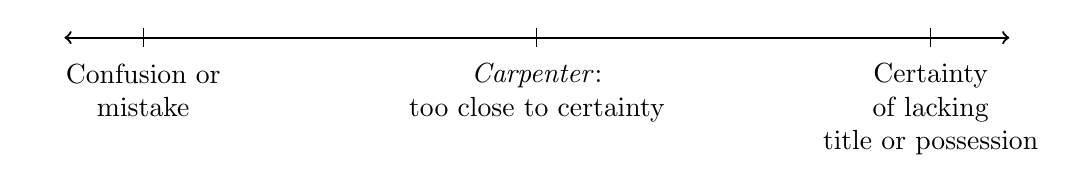
\begin{tikzpicture}
        \draw[<->, thick] (0,0) -- (12,0);
        \foreach \x in {1,6,11} {
            \draw (\x,0.12) -- (\x,-0.12);
        }

        \node[
            below=6pt,
            text width=2.7cm,
            align=center
        ] at (1,0) {
            Confusion or\\
            mistake
        };

        \node[
            below=6pt,
            text width=3.5cm,
            align=center
        ] at (6,0) {
            \textit{Carpenter}:\\
            too close to certainty
        };

        \node[
            below=6pt,
            text width=3cm,
            align=center
        ] at (11,0) {
            Certainty of lacking\\
            title or possession
        };
    \end{tikzpicture}
\end{center}

\subsection{Adverse Possession Against the Government}

\rulebox{Adverse Possession Against the Government}{
The traditional rule is that adverse possession does not run against the government. A government-owned parcel generally cannot be acquired through adverse possession unless a statute expressly provides otherwise.
}

\note{Rationale}{
\begin{itemize}
    \item The government owns land on behalf of the public.
    \item Allowing private parties to acquire public land through adverse possession could harm the public without effective notice to the relevant government entity.
    \item The rule also reflects sovereign immunity and the difficulty of monitoring all government-owned property.
\end{itemize}
}

\subsection{Tacking and Continuity}

\casebox
{\textit{Howard v. Kunto} (1970)}
{}
{
\textbf{Facts}
\begin{itemize}
    \item Kunto occupied a waterfront vacation home that was technically located on a neighboring owner's lot because of a surveying error.
    \item Kunto and his predecessors had occupied the property primarily during the summer.
\end{itemize}

\textbf{Questions}
\begin{itemize}
    \item Did seasonal use satisfy the continuity requirement?
    \item Could Kunto tack his predecessors' periods of possession?
\end{itemize}

\textbf{Holding}
\begin{itemize}
    \item Yes. Seasonal use was continuous because it was consistent with the ordinary use of a summer home.
    \item Yes. Kunto could tack his predecessors' possession because the occupants were in privity.
\end{itemize}

\textbf{Discussion}
\begin{itemize}
    \item \textbf{Continuity:} Possession need not be constant or daily. The relevant question is how an ordinary owner would use the particular property.
    \item \textbf{Tacking:} Successive possessors may combine periods of possession when there is privity, such as a voluntary transfer by deed or sale.
    \item Tacking is not permitted when the later possessor ousts the earlier possessor or enters without a legally recognized connection.
\end{itemize}
}

\note{Two Important Concepts from \textit{Kunto}}{
\begin{enumerate}
    \item \textbf{Continuity is property-specific:} Seasonal use may be continuous when seasonal use is normal for the type of property.
    \item \textbf{Tacking requires privity:} Successive possessors may combine their periods of possession when there is a voluntary legal relationship between them.
\end{enumerate}
}

\subsection{Takeaways}{
\begin{enumerate}
    \item The standard elements are actual, exclusive, continuous, open and notorious, and hostile under a claim of right.
    \item The precise elements vary by jurisdiction. For example, some jurisdictions separately require peaceable possession.
    \item The most contested issue is often the claim-of-right requirement:
    \begin{itemize}
        \item Objective jurisdictions ask whether the possession looked like a claim of ownership.
        \item Subjective jurisdictions ask whether the possessor acted in good faith.
    \end{itemize}
    \item Adverse possession doctrines reflect recurring property-law values:
    \begin{itemize}
        \item Rewarding labor;
        \item Reducing administrative costs;
        \item Encouraging productive use;
        \item Protecting reliance; and
        \item Settling old disputes.
    \end{itemize}
\end{enumerate}
}


\chapter{Alternatives to Private Property}

\section{Limits of Private Property}

\subsection{Theoretical Perspectives}

\subsubsection{Anti-commodification}

\note{Property as a Bundle of Rights}{
\begin{itemize}
    \item Property is often described as a ``bundle of sticks'' rather than a single absolute right.
    \item The bundle may include:
    \begin{itemize}
        \item The right to exclude;
        \item The right to use;
        \item The right to transfer;
        \item The right to derive income; and
        \item The right to possess.
    \end{itemize}
    \item A limitation on one stick does not necessarily eliminate all property rights.
\end{itemize}
}

\definition{Fungible Property}
{
Property whose individual units are interchangeable and have substantially equivalent market value.
}

\note{\textit{Property and Personhood}, Radin}{
\begin{itemize}
    \item Radin distinguishes between:
    \begin{itemize}
        \item \textbf{Fungible property:} replaceable objects valued primarily through market exchange; and
        \item \textbf{Personal property:} objects connected to identity, relationships, or personal development and not fully replaceable through market value.
    \end{itemize}
    \item Property connected to personhood may deserve stronger protection than fungible property.
    \item The theory applies most naturally to objects outside the body. It does not imply that a person's body should be treated as ordinary property.
    \item The theory must distinguish genuine personhood interests from fetishization or unhealthy attachment to objects.
\end{itemize}
}

\note{Market Inalienability, Radin}{
\begin{itemize}
    \item Inalienability rules restrict the ability to sell or transfer certain goods even when the owner wishes to sell them.
    \item \textbf{Prophylactic or coercion argument:}
    \begin{itemize}
        \item Some transactions are likely to involve coercion or exploitation.
        \item Because it may be costly to determine whether every transaction was genuinely voluntary, the law may prohibit the transaction categorically.
        \item Criticism: this may be paternalistic and may prevent people from using transactions to improve their circumstances.
    \end{itemize}
    
    \item \textbf{Prohibition or moral argument:}
    \begin{itemize}
        \item Some things may be degraded or morally damaged by being treated as commodities.
        \item Market language may obscure values that should not be reduced to price.
    \end{itemize}
    
    \item \textbf{Domino argument:}
    \begin{itemize}
        \item Allowing one form of commodification may lead to the commodification of increasingly broad categories of things.
    \end{itemize}
    
    \item \textbf{Double bind:}
    \begin{itemize}
        \item Prohibiting a transaction may protect people from exploitation but also remove one avenue through which people could improve their circumstances.
    \end{itemize}
\end{itemize}
}

\question
{What are the pros and cons of inalienability rules?}
{
\begin{itemize}
    \item \textbf{Arguments for inalienability:}
    \begin{itemize}
        \item Prevents coercion and exploitation;
        \item Protects personhood interests;
        \item Preserves moral or social values; and
        \item Prevents harmful markets from expanding.
    \end{itemize}
    
    \item \textbf{Arguments against inalienability:}
    \begin{itemize}
        \item Limits individual autonomy;
        \item May be paternalistic;
        \item May prevent mutually beneficial exchanges; and
        \item May harm people who rely on the prohibited transaction.
    \end{itemize}
\end{itemize}
}


\subsubsection{The Commons}

\definition{The Tragedy of the Commons}
{
The tragedy of the commons occurs when individuals acting in their own self-interest overuse an open-access resource, causing depletion or harm to the resource as a whole.
}

\definition{Externality}
{
A cost or benefit imposed on someone who did not choose to bear or receive it as a result of another person's conduct.
}

\definition{Internalization}
{
The process of requiring the person who creates an externality to bear the costs or receive the benefits of that conduct.
}

\note{Responses to Commons Problems, Ostrom}{
\begin{enumerate}
    \item \textbf{Privatization:}
    \begin{itemize}
        \item Private ownership may cause users to internalize the costs of overuse.
        \item Downsides include the cost of creating property boundaries, unequal initial distribution, and the possibility that privatization will not address all externalities.
    \end{itemize}
    
    \item \textbf{Central authority:}
    \begin{itemize}
        \item A government or other central institution creates and enforces rules.
        \item This may be administratively effective once established, but enforcement can be costly and centralized decision-making may be poorly tailored to local conditions.
    \end{itemize}
    
    \item \textbf{Closed-access commons:}
    \begin{itemize}
        \item Access is limited to a defined group that shares rules and responsibilities.
        \item This system often relies on social norms, monitoring, and informal enforcement.
    \end{itemize}
    
    \item \textbf{Tradable access rights:}
    \begin{itemize}
        \item A central authority caps total use and allocates permits that users may buy, sell, or trade.
        \item This creates a market in access rights rather than privatizing the resource itself.
    \end{itemize}
\end{enumerate}
}

\textbf{Conditions for a Successful Closed-Access Commons}{
\begin{itemize}
    \item A relatively small and stable group of users.
    \item Shared norms and cultural expectations.
    \item A stable population.
    \item Stable demand or incentives.
    \item A shared understanding of the resource's carrying capacity.
    \item Effective monitoring and enforcement.
\end{itemize}
}

\casebox{Acheson and the Lobster Gangs}{}{
\begin{itemize}
    \item Maine lobster gangs illustrate a closed-access commons governed through informal social norms.
    \item The system was effective when:
    \begin{itemize}
        \item The groups were small;
        \item Users had stable relationships;
        \item Members took approximately what they needed; and
        \item The resource and demand were relatively stable.
    \end{itemize}
    \item The system became less stable when lobster prices increased and outsiders entered the fishery.
    \item Potential problems include:
    \begin{itemize}
        \item Lack of transparency;
        \item Violence or coercive enforcement;
        \item Exclusion of outsiders;
        \item Homogeneous or discriminatory group structures; and
        \item The possibility that marginalized users will be excluded.
    \end{itemize}
\end{itemize}
}

\casebox{The Island of Barbuda}{}{
\begin{itemize}
    \item Barbuda historically used a communal land system rather than individualized private title.
    \item After a hurricane, the government argued that formal title would allow residents to use their homes as collateral for rebuilding loans.
    \item The example illustrates the benefits and limitations of a closed-access commons:
    \begin{itemize}
        \item Communal ownership may protect community control and prevent dispossession.
        \item Lack of individualized title may limit access to credit and formal financing.
    \end{itemize}
\end{itemize}
}

\textbf{\textit{Theory of Property Rights}, Demsetz}{
\begin{itemize}
    \item Property rights emerge when the benefits of internalizing externalities exceed the costs of creating and enforcing the rights.
    \item As a resource becomes more valuable, users have a greater incentive to establish ownership rules.
    \item Demsetz's fur-trade example illustrates how increased value can lead communities to develop more exclusive property rights to prevent overhunting.
    \item Property rights may improve efficiency by aligning individual incentives with social costs and benefits.
    \item Limitations include:
    \begin{itemize}
        \item Difficulties in distributing rights initially;
        \item Costs of monitoring and enforcement;
        \item Externalities that cross property boundaries; and
        \item Large-scale problems such as climate change that private ownership alone cannot solve.
    \end{itemize}
\end{itemize}
}

\subsection{Takeaways}{
\begin{enumerate}
    \item Private property is only one way to organize control over resources.
    \item Inalienability rules limit transfer in order to protect autonomy, personhood, or social values.
    \item Privatization is only one solution to commons problems.
    \item Closed-access commons can work when communities are small, stable, and governed by shared norms.
    \item Central authority and tradable access rights offer alternative solutions, but each creates its own administrative and distributive problems.
    \item Property rules should therefore be evaluated by asking:
    \begin{itemize}
        \item Who receives the right?
        \item Who bears the costs?
        \item What values does the rule promote?
        \item What institutional structure can administer the rule?
        \item What happens to people excluded from the property system?
    \end{itemize}
\end{enumerate}
}

\end{document}
